\section{Arc Length and Surface Area} \label{S:6.3.ArcLength}

\begin{goals}
\item How can a definite integral be used to measure the length of a curve?
\item How can a definite integral be used to measure the surface area of a solid of revolution?
\end{goals}

%-------------------------------
% SUBSECTION INTRODUCTION
%-------------------------------
\subsection*{Introduction}

\begin{marginfigure}[6cm] % MARGIN FIGURE
\margingraphics{figures/6_1_Intro.eps}
\caption{The area between a nonnegative function $f$ and the $x$-axis on the interval $[a,b]$.} \label{F:6.1.Intro}
\end{marginfigure}

Early on in our work with the definite integral, we learned that if we have a nonnegative velocity function, $v$, for an object moving along an axis, the area under the velocity function between $a$ and $b$ tells us the distance the object traveled on that time interval.  Moreover, based on the definition of the definite integral, that area is given precisely by $\int_a^b v(t) \, dt$.  Indeed, for any nonnegative function $f$ on an interval $[a,b]$, we know that $\int_a^b f(x) \, dx$ measures the area bounded by the curve and the $x$-axis between $x = a$ and $x = b$, as shown in Figure~\ref{F:6.1.Intro}.

Through our upcoming work in the present section and chapter, we will explore how definite integrals can be used to represent a variety of different physically important properties.  In Preview Activity~\ref{PA:6.1}, we begin this investigation by seeing how a single definite integral may be used to represent the area between two curves.

\begin{pa} \label{PA:6.3}  In the following, we consider the function $f(x)=1-x^2$ over the interval $[-1,1]$. Our goal is to estimate the length of the curve. 

\ba
\item Graph $f(x)$ over the interval $[-1,1]$. Label the points on the curve that correspond to $x=-1,-\frac12,0,1/2$, and $1$.  

\item Draw the secant line connecting the points $(-1,f(-1)$ and \newline $(-\frac{1}{2},f(-\frac{1}{2}))$. Use the distance formula to find the length of the secant line from $x=-1$ to $x=-\frac12$.
\item Repeat drawing a secant line between the remaining points starting with $(-\frac{1}{2},f(-\frac{1}{2}))$ and $(0,f(0))$. For each line segment , use the distance formula to find the length of the segment.
\item Add the distances together to get an approximation to the length of the curve. 
\item How can we improve our approximation? Write a Riemann sum that will give an improvement to our approximation. 
\ea
\end{pa} 
\afterpa % PREVIEW 

%------------------------------------------
% SUBSECTION FINDING THE LENGTH OF A CURVE
%------------------------------------------
\subsection*{Finding the length of a curve} \index{arc length}

In addition to being able to use definite integrals to find the volumes of solids of revolution, we can also use the definite integral to find the length of a portion of a curve.  We use the same fundamental principle:  we take a curve whose length we cannot easily find, and slice it up into small pieces whose lengths we can easily approximate.  In particular, we take a given curve and subdivide it into small approximating line segments, as shown at left in Figure~\ref{F:6.3.ArcLength}.
  
\begin{marginfigure}[2cm] % MARGIN FIGURE
\margingraphics{figures/6_1_ArcLength.eps}
\caption{At left, a continuous function $y = f(x)$ whose length we seek on the interval $a = x_0$ to $b = x_3$.  At right, a close up view of a portion of the curve.} \label{F:6.3.ArcLength}
\end{marginfigure}

To see how we find such a definite integral that measures arc length on the curve $y = f(x)$ from $x = a$ to $x = b$, we think about the portion of length, $L_{\mbox{\small{slice}}}$, that lies along the curve on a small interval of length $\triangle x$, and estimate the value of $L{\mbox{\small{slice}}}$ using a well-chosen triangle.  In particular, if we consider the right triangle with legs parallel to the coordinate axes and hypotenuse connecting two points on the curve, as seen at right in Figure~\ref{F:6.3.ArcLength}, we see that the length, $h$, of the hypotenuse approximates the length, $L_{\mbox{\small{slice}}}$, of the curve between the two selected points.  Thus,
$$L_{\mbox{\small{slice}}} \approx h = \sqrt{ (\triangle x)^2 + (\triangle y)^2 }.$$
By algebraically rearranging the expression for the length of the hypotenuse, we see how a definite integral can be used to compute the length of a curve.  In particular, observe that by removing a factor of $(\triangle x)^2$, we find that
\begin{eqnarray*}
L_{\mbox{\small{slice}}} & \approx & \sqrt{ (\triangle x)^2 + (\triangle y)^2 } \\
& = & \sqrt{ (\triangle x)^2\left(1 + \frac{(\triangle y)^2}{(\triangle x)^2} \right)} \\
& = & \sqrt{1 + \frac{(\triangle y)^2}{(\triangle x)^2} } \cdot \triangle x.
\end{eqnarray*}
Furthermore, as $n \to \infty$ and $\triangle x \to 0$, it follows that $\frac{\triangle y}{\triangle x} \to \frac{dy}{dx} = f'(x)$.  Thus, we can say that
$$L_{\mbox{\small{slice}}} \approx \sqrt{1 + f'(x)^2} \triangle x.$$
Taking a Riemann sum of all of these slices and letting $n \to \infty$, we arrive at the following fact.

\concept{Arc Length}{ %CONCEPT
Given a differentiable function $f$ on an interval $[a,b]$, the total arc length\index{arc length}, $L$, along the curve $y = f(x)$ from $x = a$ to $x = b$ is given by
$$L = \int_a^b \sqrt{1+f'(x)^2} \, dx.$$
} %end CONCEPT

\begin{example} \label{eg:6.3.1} % EXAMPLE
Find the arc length of $f(x) = x^{3/2}$ from $x=0$ to $x=4$. 

\solution
We begin by finding $\fp(x)= \frac32x^{1/2}$. Using the formula, we find the arc length $L$ as
\begin{align*}
	L &=	\int_0^4 \sqrt{1+\left(\frac32x^{1/2}\right)^2}\ dx \\
		&=	\int_0^4 \sqrt{1+\frac94x} \ dx \\
		&= 	\int_0^4 \left(1+\frac94x\right)^{1/2}\ dx \\
		&=  \frac23\frac49\left(1+\frac94x\right)^{3/2}\Big|_0^4 \\
		&=\frac{8}{27}\left(10^{3/2}-1\right) \approx 9.07 \text{units}.
\end{align*}
A graph of $f$ is given in Figure \ref{F:6.3.Ex1}.
\end{example}

\begin{marginfigure}[-8cm] %MARGIN FIGURE
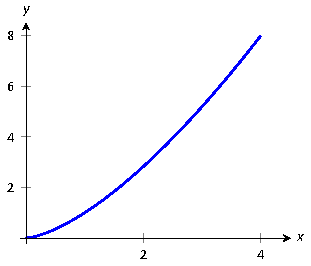
\includegraphics{figures/figarc1}
\caption{A graph of $f(x) = x^{3/2}$ from Example~\ref{eg:6.3.1}.} \label{F:6.3.Ex1}
\end{marginfigure}

 % EXAMPLE

\begin{example} \label{eg:6.3.2} % EXAMPLE
Find the arc length of $\ds f(x) =\frac18x^2-\ln x$ from $x=1$ to $x=2$.

\solution
This function was chosen specifically because the resulting integral can be evaluated exactly. We begin by finding $\fp(x) = x/4-1/x$. The arc length is 
\begin{align*}
L		&=  \int_1^2 \sqrt{1+ \left(\frac x4-\frac1x\right)^2}\ dx \\
		&= 	\int_1^2 \sqrt{1 + \frac{x^2}{16} -\frac12 + \frac1{x^2} } \ dx \\
\end{align*}
\begin{align*}
\phantom{L}
		&=	\int_1^2 \sqrt{\frac{x^2}{16} +\frac12 + \frac1{x^2} } \ dx \\
		&=	\int_1^2	\sqrt{ \left(\frac x4 + \frac1x\right)^2}\ dx \\
		&= \int_1^2 \left(\frac x4 + \frac1x\right) \ dx \\
		&=  \left(\frac{x^2}8 + \ln x\right)\Bigg|_1^2\\
		&=	\frac38+\ln 2 \approx 1.07 \ \text{units}.
\end{align*}
	
A graph of $f$ is given in Figure \ref{F:6.3.Ex2}; the portion of the curve measured in this problem is in bold.

\end{example}

\begin{marginfigure}[-8cm] %MARGIN FIGURE
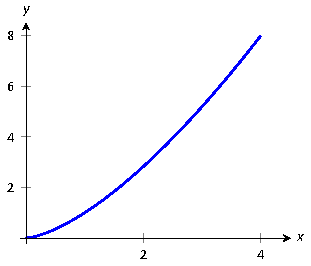
\includegraphics{figures/figarc1}
\caption{A graph of $f(x) = \frac18x^2-\ln x$ from Example~\ref{eg:6.3.2}.} \label{F:6.3.Ex2}
\end{marginfigure}

 % EXAMPLE

\begin{margintable}[3cm]
\begin{center}
\scalebox{1.15}{
\begin{tabular}{c | r} 
 $x$ & $\sqrt{1+\cos^2x}$ \\ \hline
 $0$ & $\sqrt{2}$ \\
 $\pi/4$ & $\sqrt{3/2}$ \\
 $\pi/2$ & $1$ \\
 $3 \pi/4$ & $\sqrt{3/2}$ \\
 $\pi$  & $\sqrt{2}$ \\
\end{tabular}}
\end{center}
\caption{A table of values of $y=\sqrt{1+\cos^2x}$ to evaluate a definite integral in Example \ref{eg:6.3.3}.} \label{T:6.3.Ex3}
\end{margintable}

\begin{example} \label{eg:6.3.3} % EXAMPLE
Find the length of the sine curve from $x=0$ to $x=\pi$.

\solution This is somewhat of a mathematical curiosity; in Activity \ref{A:4.5.1} (b) we found the area under one ``hump'' of the sine curve is 2 square units; now we are measuring its arc length.

The setup is straightforward: $f(x) = \sin x$ and $\fp(x) = \cos x$. Thus 
$$L = \int_0^\pi \sqrt{1+\cos^2x}\ dx.$$
This integral \textit{cannot} be evaluated in terms of elementary functions so we will approximate it with Simpson's Method with $n=4$. 

Table~\ref{T:6.3.Ex3} gives $\sqrt{1+\cos^2x}$ evaluated at 5 evenly spaced points in $[0,\pi]$. Simpson's Rule then states that 
\begin{align*}
\int_0^\pi \sqrt{1+\cos^2x}\ dx &\approx	\frac{\pi-0}{4\cdot 3}\left(\sqrt{2}+4\sqrt{3/2}+2(1)+4\sqrt{3/2}+\sqrt{2}\right) \\
			&=3.82918.
\end{align*}
Using a computer with $n=100$ the approximation is $L\approx 3.8202$; our approximation with $n=4$ is quite good.
\end{example} % EXAMPLE

\begin{activity} \label{A:6.3.1}  Each of the following questions somehow involves the arc length along a curve.
\ba
	
	\item Use the definition and appropriate computational technology to determine the arc length along $y = x^2$ from $x = -1$ to $x = 1$.
	\item Find the arc length of $y = \sqrt{4-x^2}$ on the interval $0 \le x \le 4$.  Find this value in two different ways: (a) by using a definite integral, and (b) by using a familiar property of the curve.
	\item Determine the arc length of $y = xe^{3x}$ on the interval $[0,1]$.
	\item Will the integrals that arise calculating arc length typically be ones that we can evaluate exactly using the First FTC, or ones that we need to approximate?  Why?
	\item A moving particle is traveling along the curve given by $y = f(x) = 0.1x^2 + 1$, and does so at a constant rate of 7 cm/sec, where both $x$ and $y$ are measured in cm (that is, the curve $y = f(x)$ is the path along which the object actually travels; the curve is not a ``position function'').  Find the position of the particle when $t = 4$ sec, assuming that when $t = 0$, the particle's location is $(0,f(0))$.
\ea

\end{activity}
\begin{smallhint}
\ba
	\item Small hints for each of the prompts above.
\ea
\end{smallhint}
\begin{bighint}
\ba
	\item Big hints for each of the prompts above.
\ea
\end{bighint}
\begin{activitySolution}
\ba
	\item Solutions for each of the prompts above.
\ea
\end{activitySolution}
\aftera % ACTIVITY

%-------------------------------------------------
% SUBSECTION SURFACE AREA OF SOLIDS OF REVOLUTION
%-------------------------------------------------
\subsection*{Surface Area of Solids of Revolution}

We have already seen how a curve $y=f(x)$ on $[a,b]$ can be revolved around an axis to form a solid. Instead of computing its volume, we now consider its surface area.

\begin{marginfigure}[6cm] % MARGIN FIGURE
\captionsetup[subfigure]{labelformat=empty}
\subfloat{\margingraphics{figures/figarc4b}}

\subfloat{\margingraphics{figures/figarc4}}

\caption{Establishing the formula for surface area.} \label{F:6-3_SurfArea}
\end{marginfigure}

We begin as we have in the previous sections: we partition the interval $[a,b]$ with $n$ subintervals, where the $i\,^{\text{th}}$ subinterval is $[x_i,x_{i+1}]$. On each subinterval, we can approximate the curve $y=f(x)$ with a straight line that connects $f(x_i)$ and $f(x_{i+1})$ as shown in Figure \ref{F:6-3_SurfArea} (a). Revolving this line segment about the $x$-axis creates part of a cone (called the \textit{frustum} of a cone) as shown in Figure \ref{F:6-3_SurfArea} (b). The surface area of a frustum of a cone is $$2\pi\cdot\text{ length }\cdot\text{average of the two radii $R$ and $r$}.$$

The length is given by $L$; we use the material just covered by arc length to state that $$L\approx \sqrt{1+\fp(c_i)}\dx_i$$ for some $c_i$ in the $i\,^\text{th}$ subinterval. The radii are just the function evaluated at the endpoints of the interval. That is, $$R = f(x_{i+1})\quad \text{and}\quad r = f(x_i).$$

Thus the surface area of this sample frustum of the cone is approximately 
$$2\pi\frac{f(x_i)+f(x_{i+1})}2\sqrt{1+\fp(c_i)^2}\dx_i.$$

Since $f$ is a continuous function, the Intermediate Value Theorem states there is some $d_i$ in $[x_i,x_{i+1}]$ such that \newline $\ds f(d_i) = \frac{f(x_i)+f(x_{i+1})}2$; we can use this to rewrite the above equation as
$$2\pi f(d_i)\sqrt{1+\fp(c_i)^2}\dx_i.$$
Summing over all the subintervals we get the total surface area to be approximately 
$$\text{Surface Area}\approx \sum_{i=1}^n 2\pi f(d_i)\sqrt{1+\fp(c_i)^2}\dx_i,$$
which is a Riemann Sum. Taking the limit as the subinterval lengths go to zero gives us the exact surface area, given in the following Key Idea.

\concept{Surface Area of a Solid of Revolution} %CONCEPT
{Let $f$ be differentiable on an open interval containing $[a,b]$ where $\fp$ is also continuous on $[a,b]$. \index{integration!surface area}\index{surface area!solid of revolution}
	\begin{enumerate}[1)]
	\item	The surface area of the solid formed by revolving the graph of $y=f(x)$, where $f(x)\geq0$, about the $x$-axis is
	$$\text{Surface Area} = 2\pi\int_a^b f(x)\sqrt{1+\fp(x)^2}\ dx.$$
	\item	The surface area of the solid formed by revolving the graph of $y=f(x)$ about the $y$-axis, where $a,b\geq0$, is
	$$\text{Surface Area} = 2\pi\int_a^b x\sqrt{1+\fp(x)^2}\ dx.$$
	\end{enumerate}
} %end CONCEPT

\marginnote{When revolving $y=f(x)$ about the $y$-axis, the radii of the resulting frustum are $x_i$ and $x_{i+1}$; their average value is simply the midpoint of the interval. In the limit, this midpoint is just $x$. }

\begin{example} \label{eg:6.3.4} % EXAMPLE
Find the surface area of the solid formed by revolving $y=\sin x$ on $[0,\pi]$ around the $x$-axis, as shown in Figure \ref{F:6.3.Ex4}.

\solution
The setup is relatively straightforward; we have the surface area $SA$ is:
\begin{align*}
SA  &=	2\pi\int_0^\pi \sin x\sqrt{1+\cos^2x}\ dx \\
	&= 2\pi \int_{-1}^1 \sqrt{1+u^2} \ du \\
		&=	2\pi \int_{-\pi/4}^{\pi/4} \sec^3\theta \ d\theta \\
		&= 2\pi\sqrt{2}.		
\end{align*}
The integration above is nontrivial, utilizing Substitution, Trigonometric Substitution, and Integration by Parts.
\end{example}

\begin{marginfigure}[-8cm] %MARGIN FIGURE
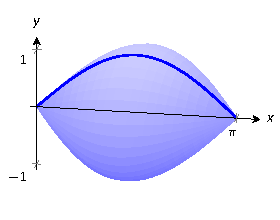
\includegraphics{figures/figsa1}
\caption{Revolving $y=\sin x$ on $[0,\pi]$ about the $x$-axis.} \label{F:6.3.Ex4}
\end{marginfigure}



 % EXAMPLE

\begin{example} \label{eg:6.3.5} % EXAMPLE
Find the surface area of the solid formed by revolving the curve $y=x^2$ on $[0,1]$ about:
\begin{enumerate}[1)]
\item the $x$-axis
\item	 the $y$-axis.
\end{enumerate}

\solution
\begin{enumerate}[1)]
\item The integral is straightforward to setup:
\begin{align*}
SA &= 2\pi\int_0^1 x^2\sqrt{1+(2x)^2}\ dx.
\intertext{Like the integral in Example \ref{eg:6.3.4}, this requires Trigonometric Substitution.}
&= \left.\frac{\pi}{32}\left(2(8x^3+x)\sqrt{1+4x^2}-\sinh^{-1}(2x)\right)\right|_0^1\\
&=\frac{\pi}{32}\left(18\sqrt{5}-\sinh^{-1}2\right)\\
&\approx 3.81\ \text{units}^2.
\end{align*}
The solid formed by revolving $y=x^2$ around the $x$-axis is graphed in Figure \ref{F:6.3.Ex5}-(a).
	
\item	 Since we are revolving around the $y$-axis, the ``radius'' of the solid is not $f(x)$ but rather $x$. Thus the integral to compute the surface area is:
\begin{align*}
SA &= 2\pi\int_0^1x\sqrt{1+(2x)^2}\ dx.
\intertext{This integral can be solved using substitution. Set $u=1+4x^2$; the new bounds are $u=1$ to $u=5$. We then have }
&=	\frac{\pi}4\int_1^5 \sqrt{u}\ du \\
&= \left.\frac{\pi}{4}\frac23 u^{3/2}\right|_1^5\\
&= \frac{\pi}6\left(5\sqrt{5}-1\right)\\
&\approx 5.33\ \text{units}^2.
\end{align*}
 The solid formed by revolving $y=x^2$ about the $y$-axis is graphed in Figure \ref{F:6.3.Ex5}-(b).	
\end{enumerate}
\end{example}

\begin{marginfigure}[-15cm] %MARGIN FIGURE
%\captionsetup[subfigure]{labelformat=empty}
\subfloat[]{\margingraphics{figures/figsa2a}}

\vspace{1cm}

\subfloat[]{\margingraphics{figures/figsa2b}}

\caption{The solids used in Example \ref{eg:6.3.5}} \label{F:6.3.Ex5}
\end{marginfigure}



 % EXAMPLE

This last example is a famous mathematical ``paradox.''

\begin{example} \label{eg:6.3.6} % EXAMPLE
%\textbf{The surface area and volume of Gabriel's Horn} 

Consider the solid formed by revolving $y=1/x$ about the $x$-axis on $[1,\infty)$. Find the volume and surface area of this solid. (This shape, as graphed in Figure \ref{F:6.3.Ex6}, is known as ``Gabriel's Horn'' since it looks like a very long horn that only a supernatural person, such as an angel, could play.)\index{Gabriel's Horn}

\solution
To compute the volume it is natural to use the Disk Method. We have:
\begin{align*}
V &= \pi\int_1^\infty \frac{1}{x^2}\ dx \\
	&= \lim_{b\to\infty}\pi\int_1^b\frac{1}{x^2}\ dx \\
	&=	\lim_{b\to\infty} \left.\pi\left(\frac{-1}{x}\right)\right|_1^b \\
	&= \lim_{b\to\infty} \pi\left(1-\frac1b\right) \\
	&= \pi \ \text{units}^3.
\end{align*}
Gabriel's Horn has a finite volume of $\pi$ cubic units. Since we have already seen that objects with infinite length can have a finite area, this is not too difficult to accept.

We now consider its surface area. The integral is straightforward to setup:
\begin{align*}
SA &= 2\pi\int_1^\infty \frac{1}{x}\sqrt{1+1/x^4}\ dx.
\intertext{Integrating this expression is not trivial. We can, however, compare it to other improper integrals. Since $1< \sqrt{1+1/x^4} $ on $[1,\infty)$, we can state that}
2\pi\int_1^\infty \frac{1}{x}\ dx &<2\pi\int_1^\infty \frac{1}{x}\sqrt{1+1/x^4}\ dx .
\end{align*}
The improper integral on the left diverges. Since the integral on the right is larger, we conclude it also diverges, meaning Gabriel's Horn has infinite surface area.

Hence the ``paradox'': we can fill Gabriel's Horn with a finite amount of paint, but since it has infinite surface area, we can never paint it.

Somehow this paradox is striking when we think about it in terms of volume and area. However, we have seen a similar paradox before, as referenced above. We know that the area under the curve $y=1/x^2$ on $[1,\infty)$ is finite, yet the shape has an infinite perimeter. Strange things can occur when we deal with the infinite.

\end{example}

\begin{marginfigure}[-8cm] %MARGIN FIGURE
\margingraphics{figures/figgabriel}
\caption{A graph of Gabriel's Horn.} \label{F:6.3.Ex6}
\end{marginfigure}



 % EXAMPLE

%--------------------------------------------
% SUMMARY
%--------------------------------------------
\begin{summary}
  \item To find the area between two curves, we think about slicing the region into thin rectangles.  If, for instance, the area of a typical rectangle on the interval $x = a$ to $x = b$ is given by $A_{\mbox{\small{rect}}} = (g(x) - f(x)) \triangle x,$ then the exact area of the region is given by the definite integral
  $$A = \int_a^b (g(x)-f(x))\, dx.$$
  \item The shape of the region usually dictates whether we should use vertical rectangles of thickness $\triangle x$ or horizontal rectangles of thickness $\triangle y$.  We desire to have the height of the rectangle governed by the difference between two curves:  if those curves are best thought of as functions of $y$, we use horizontal rectangles, whereas if those curves are best viewed as functions of $x$, we use vertical rectangles.
  \item The arc length, $L$, along the curve $y = f(x)$ from $x = a$ to $x = b$ is given by
$$L = \int_a^b \sqrt{1 + f'(x)^2} \, dx.$$
\end{summary}

\clearpage

%--------------
% EXERCISES
%--------------
\begin{adjustwidth*}{}{-2.25in}
\textbf{{\large Exercises}}
\setlength{\columnsep}{25pt}
\begin{multicols*}{2}
\noindent Terms and Concepts \small
\begin{enumerate}[1)]
\item T/F: The integral formula for computing Arc Length was found by first approximating arc length with straight line segments.
\item T/F: The integral formula for computing Arc Length includes a square--root, meaning the integration is probably easy.
\end{enumerate} 

\noindent {\normalsize Problems} \small

\noindent{\bf In Exercises 3--11, find the arc length of the function on the given integral.}

\begin{enumerate}[1),resume]
\item $\ds f(x) = x$ on $[0, 1]$
\item $\ds f(x) = \sqrt{8x}$ on $[-1, 1]$
\item $\ds f(x) = \frac13x^{3/2}-x^{1/2}$ on $[0,1]$
\item $\ds f(x) = \frac1{12}x^{3}+\frac1x$ on $[1,4]$
\item $\ds f(x) = 2x^{3/2}-\frac16\sqrt{x}$ on $[0,9]$
\item $\ds f(x) = \frac12\big(e^x+e^{-x}\big)$ on $[0, \ln 5]$
\item $\ds f(x) = \frac1{12}x^5+\frac1{5x^3}$ on $[.1, 1]$
\item $\ds f(x) = \ln \big(\sin x\big)$ on $[\pi/6, \pi/2]$
\item $\ds f(x) = \ln \big(\cos x\big)$ on $[0, \pi/4]$
\end{enumerate}

\noindent{\bf In Exercises 12--19, set up the integral to compute the arc length of the function on the given interval. Try to compute the integral by hand, and use a CAS to compute the integral.  Also, use Simpson's Rule with $n = 4$ to approximate the arc length.}

\begin{enumerate}[1),resume]
\item $\ds f(x) = x^2$ on $[0, 1]$.\label{ex_07_04_ex_13}
\item $\ds f(x) = x^{10}$ on $[0, 1]$
\item $\ds f(x) = \sqrt{x}$ on $[0, 1]$
\item $\ds f(x) = \ln x$ on $[1, e]$
\item $\ds f(x) = \sqrt{1-x^2}$ on $[-1, 1]$. (Note: this describes the top half of a circle with radius 1.)
\item $\ds f(x) = \sqrt{1-x^2/9}$ on $[-3, 3]$. (Note: this describes the top half of an ellipse with a major axis of length 6 and a minor axis of length 2.)
\item $\ds f(x) = \frac1x$ on $[1,2]$
\item $\ds f(x) = \sec x$ on $[-\pi/4,\pi/4]$.\label{ex_07_04_ex_20}
\end{enumerate}

\columnbreak

\noindent{\bf In Exercises 20--24, find the surface area of the described solid of revolution.}

\begin{enumerate}[1),resume]
\item The solid formed by revolving $y=2x$ on $[0,1]$ about the $x$-axis.
\item The solid formed by revolving $y=x^2$ on $[0,1]$ about the $y$-axis.
\item The solid formed by revolving $y=x^3$ on $[0,1]$ about the $x$-axis.
\item The solid formed by revolving $y=\sqrt{x}$ on $[0,1]$ about the $x$-axis.
\item The sphere formed by revolving $y=\sqrt{1-x^2}$ on $[-1,1]$ about the $x$-axis.
\end{enumerate}

%------------------------------------------
% END OF EXERCISES ON FIRST PAGE
%------------------------------------------
\end{multicols*}
\end{adjustwidth*}

%\clearpage
%
%\begin{adjustwidth*}{}{-2.25in}
%\setlength{\columnsep}{25pt}
%\begin{multicols*}{2}\small
%
%\begin{enumerate}[1),start=12]
%
%\end{enumerate}
%
%%---------------------------------------------
%% END OF EXERCISES ON SECOND PAGE
%%---------------------------------------------
%\end{multicols*}
%\end{adjustwidth*}

\afterexercises 

\cleardoublepage